% Designed by ruifengx

\ExplSyntaxOn
\NewDocumentCommand{\textsmallcaps}{ m }{% Define new command with one mandatory argument
  \textapperance_smallcaps:n { #1 }% Call
}%
\tl_new:N \l__textapperance_textsmallcaps_input_tl% Initialize string variable
\cs_new_protected:Npn \textapperance_smallcaps:n #1
{% Create hidden command with one argument
  \tl_set:Nx \l__textapperance_textsmallcaps_input_tl { #1 } % Fully expand contents and store them in the variable
  \regex_replace_all:nnN
  { ([^A-Z]+) }
  { \c{textscale}\cB\{0.7\cE\}\cB\{\c{uppercase}\cB\{\0\cE\}\cE\} }
  \l__textapperance_textsmallcaps_input_tl % Replace everything thats NOT a capital letter by \textsmaller[2]{\uppercase{<match>}}
  \tl_use:N \l__textapperance_textsmallcaps_input_tl   % Return
}
\ExplSyntaxOff

\beamertemplatenavigationsymbolsempty
\usebackgroundtemplate{%
  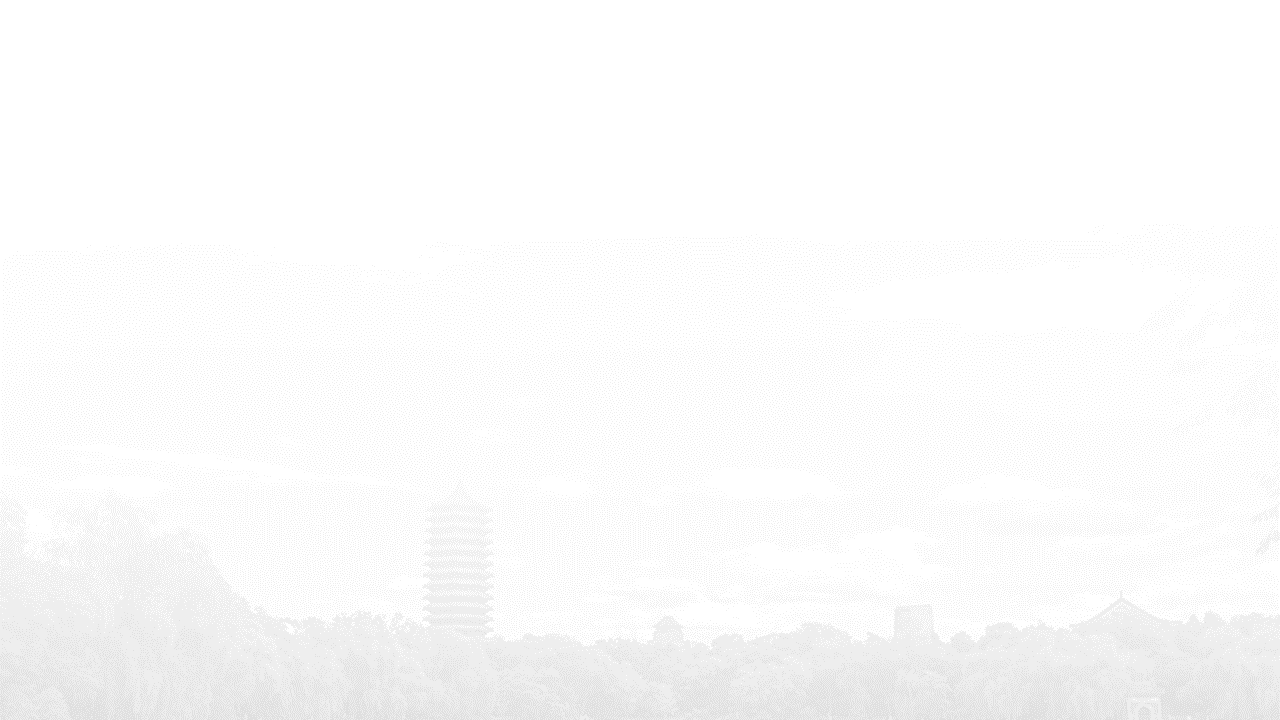
\includegraphics[width=\paperwidth,height=\paperheight]{themes/pku/background.png}%
}
\addtobeamertemplate{headline}{%
  \setlength\unitlength{1ex}%
  \begin{picture}(0,0)
    % \put{} defines the position of the frame
    \put(136,-15){\makebox(0,0)[bl]{
        
\includegraphics[height=3.5em]{themes/pku/pkulogo.pdf}
      }}%
  \end{picture}%
}{}
\usepackage{pifont}

\makeatletter
\newlength{\xrftheme@progressinheadfoot}
\newlength{\xrftheme@progressinheadfoot@linewidth}
\setlength{\xrftheme@progressinheadfoot@linewidth}{1.5pt}
\setbeamertemplate{progress bar in head/foot}{
  \nointerlineskip
  \setlength{\xrftheme@progressinheadfoot}{%
    \paperwidth * \ratio{\insertframenumber pt}{\insertmainframenumber pt}%
  }%
  \begin{beamercolorbox}[wd=\paperwidth]{progress bar in head/foot}
    \begin{tikzpicture}
      % \fill[bg] (0,0) rectangle (\paperwidth, \xrftheme@progressinheadfoot@linewidth);
      \fill[fg] (0,0) rectangle (\xrftheme@progressinheadfoot, \xrftheme@progressinheadfoot@linewidth);
    \end{tikzpicture}%
  \end{beamercolorbox}
}
\setbeamertemplate{footline}{%
  \begin{beamercolorbox}[wd=\textwidth, sep=3ex]{footline}%
    \hfill\insertframenumber
  \end{beamercolorbox}%
  \usebeamercolor*[fg]{structure}
  \usebeamertemplate*{progress bar in head/foot}%
}
\makeatother

% The \instructor command
\makeatletter
\def\instructor{\@dblarg\beamer@instructor}
\long\def\beamer@instructor[#1]#2{%
  \def\insertinstructor{\def\inst{\beamer@insttitle}\def\and{\beamer@andtitle}#2}%
  \def\beamer@shortinstructor{#1}%
}
\newcommand\insertshortinstructor[1][]{%
  {%
      \def\inst{\beamer@instother}\def\and{\beamer@andother}\let\thanks=\@gobble%
      \beamer@setupshort{#1}%
      \beamer@insertshort{\beamer@shortinstructor}%
    }}
\makeatother

\setbeamerfont{frametitle}{series=\bfseries}
\setbeamertemplate{frametitle}{
  \vspace{2.6ex}\insertframetitle\par
}
\makeatletter
\renewcommand{\maketitle}{\ifbeamer@inframe\titlepage\else\frame[plain,noframenumbering]{\titlepage}\fi}
\makeatother
\setbeamertemplate{title page}{
  \centering
  
\includegraphics[height=0.15\textheight]{themes/pku/pkulogo.pdf}
  \vfill
  \textbf{\Large \inserttitle}\\[0.8em]
  \textbf{\small \insertsubtitle}
  \vfill\small
  \insertauthor\\[0.5em]
  \insertinstitute
  \vfil
}
\setbeamertemplate{section page}{
  \vfill
  \LARGE
  {\color{darkgray}PART \insertsectionnumber}\par
  \Huge
  \vspace{-20pt}
  \setlength{\unitlength}{1ex}
  \begin{picture}(2,0)
    \thicklines
    \put(0.1,0){\color{pkured}\line(1,0){5}}
  \end{picture}\par
  \vspace{-1pt}
  {\color{pkured}\bfseries\insertsection}
  \vfill
}
\AtBeginSection{%
  \frame{\sectionpage}
}

\definecolor{pkured}{cmyk}{0,1.00,1.00,0.45}
\definecolor{pkublue}{cmyk}{1.00,0.34,0,0.45}
\definecolor{pkugreen}{cmyk}{1.00,0,0.87,0.45}
\definecolor{softgreen}{RGB}{0,176,0}
\definecolor{softblue}{RGB}{0,157,255}
\setbeamercolor{titlelike}{fg=pkured}
\setbeamercolor{subtitle}{fg=pkured}
\setbeamercolor{institute}{fg=black}
\setbeamercolor{structure}{fg=pkured}
\setbeamercolor{normal text}{fg=black}
\setbeamercolor{alerted text}{fg=pkured}
\setbeamercolor{example text}{fg=pkublue}
